\documentclass[12pt]{article}%{amsart}
\usepackage{amsmath,amssymb,latexsym,amsthm}

\numberwithin{equation}{section}% Equation numbered by section

\usepackage{geometry}
\geometry{margin=4cm}% Adjusted to make HOX readable-2cm Normal

\usepackage[T1]{fontenc}% Better text

\usepackage{graphicx}% Included for figures

\usepackage[notref,notcite]{showkeys}% add 'final' inside[]

\usepackage[toc,page]{appendix}%A ppendix sectioning
\usepackage[linktoc=all]{hyperref}% Links within document
\hypersetup{
    pdftoolbar=true,
    pdfmenubar=true,
    colorlinks,
    citecolor=violet,
    filecolor=black,
    linkcolor=violet,
    urlcolor=black
}

\usepackage[noabbrev,capitalize,nameinlink]{cleveref}%Gives correct theorem names when linking.  Use \cref{}

\usepackage{dsfont}% Used for \id                             
\usepackage{mathrsfs}% Used for \mathscr
\usepackage{tensor}% Tensor indices	
\usepackage{comment}% Commenting large sections
\usepackage{enumerate}% Enumerate options
\usepackage{mathtools}% Multilines environment
\usepackage{tcolorbox}% Boxed notes	
\usepackage{color}% Color words for clarification
\usepackage{soul}% Strike through text	
\usepackage{accents}% For \accentset										

\usepackage{tikz}
\usetikzlibrary{matrix,arrows,decorations.pathmorphing}
\tikzset{node distance=4cm, auto}









\newtheorem{thm}{Theorem}[section]
\newtheorem{prop}[thm]{Proposition}
\newtheorem{cor}[thm]{Corollary}
\newtheorem{lem}[thm]{Lemma}
\newtheorem{defn}[thm]{Definition}
\newtheorem{ex}[thm]{Example}
\newtheorem{remark}[thm]{Remark}
\newtheorem{prob}[thm]{Problem}
\newtheorem{conj}[thm]{Conjecture}

\renewenvironment{proof}{{\noindent\bfseries Proof:}}{\qed}

\begin{comment}
\begin{center}
	\begin{tikzpicture}[auto, node distance=3cm]
		\node(A){};
		\node(B)[right of=A]{};
		\node(C)[below of=A]{};
		\node(D)[right of=C]{};
		\draw[->](A) to node{}(B);
		\draw[->](A) to node[swap]{}(C);
		\draw[->](B) to node{}(D);
		\draw[->](C) to node[swap]{}(D);
	\end{tikzpicture}
\end{center}

\begin{center}
	\begin{tikzpicture}[auto, node distance=3cm]
		\node(A){};
		\node(B)[right of=A]{};
		\node(C)[right of=B]{};
		\node(D)[right of=C]{};
		\node(E)[right of=D]{};
		\draw[->](A) to node{}(B);
		\draw[->](B) to node{}(C);
		\draw[->](C) to node{}(D);
		\draw[->](D) to node{}(E);
	\end{tikzpicture}
\end{center}
	
\end{comment}







\input{../../texInput/Shortcuts.tex}

\title{Fiber Bundles}
\author{Matt Robinson}
%\author{}
\date{}

\begin{document}
	\maketitle
	\tableofcontents
	

	



%%%%%
\section{Vector Bundles}
\begin{tcolorbox}
Introductory definitions follow from \cite{kolar1999natural}, \cite{lee2003smooth}, \cite{ryan2014geometry}.

Check out \cite{borisenko1991riemannian}
\end{tcolorbox}


Let $M$ be a topological space.  A \textit{real vector bundle of rank $k$ over $M$} is a topological space $E$ together with surjective map $\pi:E\to M$ satisfying the following conditions
\begin{enumerate}[a.]
	\item For each $p\in M$, the fiber $E_p:=\pi^{-1}(p)$ over $p$ is endowed with the structure of a $k$-dimensional, real vector space.
	\item For each $p\in M$, there exists a neighborhood $U\subseteq M$ of $p$, and a homeomorphism $\Phi:\pi^{-1}(U)\to U\times\R^k$ (called the \textit{local trivialization of $E$ over $U$}) satisfying the following conditions:
		\begin{enumerate}[i.]
			\item $\pi_U\circ\Phi=\pi$ (where $\pi_U:U\times\R^k\to U$ is the projection onto $U$), and
			\item for each $q\in U$, the restriction of $\Phi$ to $E_q$ is a vector space isomorphism from $E_q$ to $\{q\}\times\R^k\cong\R^k$.
		\end{enumerate}
\end{enumerate}

If $M$ and $E$ are smooth manifolds (with or without boundary), $\pi:E\to M$ is smooth, and the local trivialization can be chosen to be diffeomorphisms, then $\pi:E\to M$ is a \textit{smooth vector bundle}.  We also call any local trivialization that is a diffeomorphism onto its image a \textit{smooth local trivialization}.  We write $\mathcal{E}$ or $(E,\pi,M)$ to denote smooth vector bundles.

We say that $E$ is the \textit{total space}, $M$ is the \textit{base space}, and $\pi$ is the \textit{projection}.  If there exists a local trivialization of $E$ over all $M$, then we that $E$ is the \textit{trivial bundle}, and have that $E$ is homeomorphic to $M\times\R^k$.  If $E$ is \textit{smoothly trivial}, then $E$ is diffeomorphic to $M\times\R^k$.  


\paragraph{Alternative Definition:}
Perhaps a better working definition for vector bundles can be described as follows.  First note, that since we're mostly interested in the smooth category, we shall ignore topological vector bundles.

Let $\pi:E\to M$ be a smooth mapping between smooth manifolds.  A \textit{vector bundle chart} on $(E,\pi, M)$ is a pair $(U,\psi)$, where $U\subseteq M$ is an open subset and $\psi$ is a fiber-respecting diffeomorphism so the following diagram commutes
\begin{center}
	\begin{tikzpicture}[auto, node distance=3cm]
		\node(A){$\rest{E}_U:=\pi^{-1}(U)$};
		\node(B)[right of=A]{};
		\node(C)[right of=B]{$U\times V$};
		\node(D)[below of=B]{$U$};
		\draw[->](A) to node{$\psi$}(C);
		\draw[->](A) to node[swap]{$\pi$}(D);
		\draw[->](C) to node{$\pi_U$}(D);
	\end{tikzpicture}
\end{center}
where $V=\pi^{-1}(p)$ is some fixed (real) $k$-dimensional vector space called the \textit{standard fiber} and $\pi_U:U\times V\to U$ is the projection onto the first factor.

Given two vector bundle charts $(U_\alpha,\psi_\alpha)$ and $(U_\beta,\psi_\beta)$, we say they are \textit{compatible} if $\psi_\alpha\circ\psi_\beta^{-1}$ is fiber-wise linear isomorphism, i.e.,
$$\psi_\alpha\circ\psi_\beta^{-1}(p,v)=(p,\psi_{\alpha\beta}(p)v),$$
for some mapping
$$\psi_{\alpha\beta}:U_{\alpha\beta}:=U_\alpha\cap U_\beta\to GL(V).$$
The mapping $\psi_{\alpha\beta}$ is then unique and smooth, and is called the \textit{transition function} between the two bundle charts.

A \textit{vector bundle atlas} $\{(U_\alpha,\psi_\alpha)\}$ for $(E,\pi, M)$ is a set of pairwise compatible bundle charts such that $\{U_\alpha\}$ is an open cover of $M$.  Two vector bundle atlases are \textit{equivalent} if their union is again a vector bundle atlas.

Thus a vector bundle $(E,\pi, M)$ consists of the smooth mapping $\pi:E\to M$ between smooth manifolds with an equivalence class of vector bundle atlases.

\begin{cor}
    Given a vector bundle $\pi:E\to M$, it follows that $\pi$ is a surjective submersion.
\end{cor}

A \textit{local section} of a smooth vector bundle $\pi:E\to M$ is a smooth map $\xi:U\to E$ for some open $U\subset M$ such that $\pi\circ\xi=\id_U$.  A \textit{(global) section} is one where $U=M$.  The \textit{zero section} is the section $\iota:M\to E$ defined by
$$\iota(p)=0_p\in E_p,$$
for each $p\in M$.  We denote the space of global sections by $\Gamma(E)$, and the space of local sections by $\Gamma(\rest{E}_U)$ (this notation will become more clear once we define the restriction of a bundle).

Given two smooth bundles $(E,\pi,M)$ and $(E',\pi',M')$, a smooth map $F:E\to E'$ is a \textit{bundle homomorphism} if there exists $f:M\to M'$ such that the following diagram commutes:
\begin{center}
	\begin{tikzpicture}[auto, node distance=3cm]
		\node(A){$E$};
		\node(B)[right of=A]{$E'$};
		\node(C)[below of=A]{$M$};
		\node(D)[right of=C]{$M'$};
		\draw[->](A) to node{$F$}(B);
		\draw[->](A) to node[swap]{$\pi$}(C);
		\draw[->](B) to node{$\pi'$}(D);
		\draw[->](C) to node[swap]{$f$}(D);
	\end{tikzpicture}
\end{center}
and $F$ is a fiber-respecting, fiber-linear map, i.e., $F_p:E_p\to E'_{f(p)}$ is linear.  Note that this implies $f$ is smooth since $f=\pi'\circ F\circ\iota$.  A bijective bundle homomorphism that's inverse is also a bundle homomorphism is called a \textit{bundle isomorphism}.  If $E$ and $E'$ are bundles over the same base space $M$, then we say a \textit{bundle homomorphism over $M$}.





%%%%%
\subsection{Operations on Vector Bundles}

\paragraph{Whitney Sums}
Suppose $E^1\to M$ and $E^2\to M$ are smooth vector bundles of rank $k_1$ and $k_2$, respectively.  Then for each $p\in M$, we have the vector space direct sum
$$E_p^1\oplus E_p^2,$$
and we define the space
$$E=E^1\oplus E^2:=\coprod_{p\in M}\left(E_p^1\oplus E_p^2\right).$$
Letting $\pi:E\to M$ denote the obvious projection, we have a new smooth vector bundle $\pi:E\to M$ called the \textit{Whitney sum of $E^1$ and $E^2$}.


\paragraph{Subbundles}
A \textit{vector subbundle} $(F,\pi, M)$ of a vector bundle $(E,\pi,M)$ is a vector bundle and vector bundle homomorphism $\phi:F\to E$ which coves $\id_M$ such that $\phi_p:F_p\to E_p$ is a linear embedding for each $p\in M$.

\begin{lem}
    Let $\phi:(E,\pi,M)\to(E',\pi',M')$ be a bundle homomorphism such that $\text{rank}(\phi_x)$ is constant in $x\in M$.  Then $\ker{\phi}$, given by $(\ker{\phi})_x=\ker{\phi_x}$ is a vector subbundle of $(E,\pi,M)$.
\end{lem}



\paragraph{Bundle Restrictions}
If $\pi:E\to M$ is a smooth vector bundle, and $A\subset M$ is any immersed submanifold of $M$, then we define the \textit{restriction of $E$ to $A$} to be the set
$$\rest{E}_A=\bigcup_{a\in A}E_a,$$
and we have a new smooth vector bundle
$$\rest{\pi}_A:\rest{E}_A\to A.$$

If $i:A\hookrightarrow M$ is an immersed submanifold, then the inclusion $i_\#:\rest{E}_A\hookrightarrow E$ is a bundle homomorphism covering $i$:
\begin{center}
	\begin{tikzpicture}[auto, node distance=3cm]
		\node(A){$\rest{E}_A$};
		\node(B)[right of=A]{$E$};
		\node(C)[below of=A]{$A$};
		\node(D)[right of=C]{$M$};
		\draw[->](A) to node{$i_\#$}(B);
		\draw[->](A) to node[swap]{$\rest{\pi}_A$}(C);
		\draw[->](B) to node{$\pi$}(D);
		\draw[->](C) to node[swap]{$i$}(D);
	\end{tikzpicture}
\end{center}

To further the understanding of the restriction of a bundle, we introduce the notion of a pullback bundle.  Let $\pi:E\to M$ be a smooth vector bundle, and $f:A\to M$ a smooth map of smooth manifolds.  The \textit{pullback bundle of $E$ along $f$} is the vector bundle $f^*\pi:f^*E\to A$ given by
$$f^*E=\{(a,(x,v))\in A\times E:f(a)=\pi(x,v)=x\},$$
and the bundle projection $f^*\pi:f^*E\to A$ is the projection onto the first factor of $A\times E$.  Then we have the vector space isomorphism
$$f^*E_a\cong E_{f(a)}.$$
Moreover, the projection onto the second factor, called the \textit{pushforth of $f$,} $f_\#:f^*E\to E$ yields the commutative diagram
\begin{center}
	\begin{tikzpicture}[auto, node distance=3cm]
		\node(A){$f^*E$};
		\node(B)[right of=A]{$E$};
		\node(C)[below of=A]{$A$};
		\node(D)[right of=C]{$M$};
		\draw[->](A) to node{$f_\#$}(B);
		\draw[->](A) to node[swap]{$f^*\pi$}(C);
		\draw[->](B) to node{$\pi$}(D);
		\draw[->](C) to node[swap]{$f$}(D);
	\end{tikzpicture}
\end{center}
Let $X\in\Gamma(f^*E)$, then the pushforth of $X$ along $f$ is the map 
$$\tilde{X}=f_\#X:A\to E$$
and the space of all sections along $f$ is denoted $\Gamma_f(E)=f_\#\Gamma(f^*E).$


In the setting of pullbacks, we let $i:A\hookrightarrow M$ be an immersed submanifold.  Then the pullback bundle
\begin{align*}
	i^*E&=\{(a,(x,v))\in A\times E:i(a)=\pi(x,v)=x\}\\
	&=\{(a,(i(a),v))\in A\times E\}\\
	&\cong\{(i(a),v)\in E:a\in A\}\\
	&=\rest{E}_A,
\end{align*}
and hence leads to the notation of $i_\#:\rest{E}_A\hookrightarrow E$ being the inclusion.


\paragraph{Lifts}
Let $\pi:E\to M$ be a smooth vector bundle and let $\gamma:I\to M$ be curve with $0,1\in I$ and $\gamma(0)=p,$ $\gamma(1)=q$.  Let $c:I\to\gamma^*E$ be a section of the pullback bundle $\gamma^*\pi:\gamma^*E\to I$.  Then the pushforth $\gamma_\#c:I\to E$ is a path in $E$ that satisfies
$$\pi\circ\gamma_\#c=\gamma.$$
That is, for the curve $\tilde{\gamma}:=\gamma_\#c$, the following diagram commutes
\begin{center}
	\begin{tikzpicture}[auto, node distance=4cm]
		\node(A){$\gamma^*E$};
		\node(B)[right of=A]{$E$};
		\node(C)[below of=A]{$I$};
		\node(D)[right of=C]{$M$};
		\draw[->](A) to node{$\gamma_\#$}(B);
		\draw[->](C) to node{$c$}(A);
		\draw[->](B) to node{$\pi$}(D);
		\draw[->](C) to node[swap]{$\gamma$}(D);
		\draw[->](C) to node{$\tilde{\gamma}$}(B);
	\end{tikzpicture}
\end{center}
The path $\tilde{\gamma}$ is called a \textit{lift of $\gamma$}.  A lift of $\gamma$ is dependent on choice of section $c\in\Gamma(\gamma^*E)$, and hence we denote the space of all lifts along $\gamma$ as $\Gamma_\gamma(E)=\gamma_\#\Gamma(\gamma^*E)$.  Note that if $\gamma$ has a self-intersection, then the lift is not a section of $E$ along $\gamma$ (despite the notational similarities).
	



%%%%%
\section{Examples of Vector Bundles}

In this section we construct in detail many of the most common smooth vector bundles in connection to smooth manifolds.  The most obvious first choice is the tangent bundle.



%%%%




%%%%%
\subsection{The Tangent Bundle}

\TOX{
See \cite{lee2003smooth} 
}

Let $M$ be a smooth $n$-dimensional manifold.  Let
$$TM=\coprod_{p\in M}T_pM,$$
denote the ``\textit{tangent bundle}''.  Let $\pi:TM\to M$, $\pi(p,v)=p$.  Then $TM$ has a natural topology and smooth structure that makes $TM$ into a smooth $2n$-dimensional manifold, and with respect to this structure, the map $\pi:TM\to M$ is smooth.

Let $(\phi,U)$ be a chart on $M$ with coordinates $(x^j)$.  Define the map $\tilde{\phi}:\pi^{-1}(U)\to\R^{2n}$ by
$$\tilde{\phi}\left(v^j\rest{\pfrac{}{x^j}}_p\right)=(x^1(p),...,x^n(p),v^1,...,v^n).$$
Its image set is $\phi(U)\times\R^n$ and is a bijection, since it's inverse can explicitly be written as
$$\tilde{\phi}^{-1}(x^1,,,,x^n,v^1,...,v^n)=v^j\rest{\pfrac{}{x^j}}_{\phi^{-1}(x)}.$$

Suppose we are given two charts $(\phi,U)$ and $(\psi,V)$ on $M$ with corresponding $(\tilde{\phi},\pi^{-1}(U))$ and $(\tilde{\psi},\pi^{-1}(V))$ on $TM$.  Then the sets
$$\tilde{\phi}(\pi^{-1}(U)\cap\pi^{-1}(V))=\phi(U\cap V)\times\R^n$$
and
$$\tilde{\psi}(\pi^{-1}(U)\cap\pi^{-1}(V))=\psi(U\cap V)\times\R^n$$
are open in $\R^{2n}$.  The transition map
$$\tilde{\psi}\circ\tilde{\phi}^{-1}:\phi(U\cap V)\times\R^n\to\psi(U\cap V)\times\R^n,$$
can then be explicitly written as
$$\tilde{\psi}\circ\tilde{\phi}^{-1}(x^1,...,x^n,v^1,...,v^n)=\left(\tilde{x}^1(x),...,\tilde{x}^n(x),v^j\pfrac{\tilde{x}^1}{x^j}(x),...,v^j\pfrac{\tilde{x}^n}{x^j}(x)\right),$$
which is clearly smooth.

Let $\{U_j\}$ be a countable cover of charts for $M$, the $\{\pi^{-1}(U_j)\}$ is a countable cover of charts for $TM$, and hence $TM$ is a smooth $2n$-dimensional manifold.

To show that $\pi:TM\to M$ is smooth, fix some local coordinates and observe that $\pi(x,v)=x$ which is clearly smooth.  Moreover, we have that $\pi:TM\to M$ is a submersion.  Since $\pi$ is a submersion if and only if every point in $TM$ is the image of a smooth local section, we fix $(p,v)\in TM$ and chart about $p$, and define the section $X:U\to TU$ by $X(q)=(q,\rest{v^j\pfrac{}{x^j}}_q)$.

We now show that $\pi:TM\to M$ is smooth vector bundle of rank $n$.  Clearly each $T_pM$ is an $n$-dimensional vector space by construction.  Fix a coordinate chart $(\phi, U)$ on $M$ and corresponding $(\tilde{\phi},\pi^{-1}(U))$ on $TM$.  Define the map $\Phi:\pi^{-1}(U)\to U\times\R^n$ by
$$\Phi\left(v^j\rest{\pfrac{}{x^j}}_p\right)=(p,(v^1,...,v^n)).$$
Then $\pi_U\circ\Phi=\pi$ and is clearly linear on each $T_pM$.  Moreover, since
$$\phi\times\id_{\R^n}\circ\Phi:\pi^{-1}(U)\to\phi(U)\times\R^n,$$
is our usual chart map $\tilde{\phi}$ on $TM$, it's a diffeomorphism, and hence $\Phi=(\phi^{-1}\times\id_{\R^n})\circ\tilde{\phi}$ is a diffeomorphism as well, and hence $\{(\pi^{-1}(U),\Phi)\}$ is our desired vector bundle atlas.















\begin{comment}

%%%%
\subsection{The Cotangent Bundle}




%%%%
\subsection{The Tensor Bundle}




%%%%
\subsection{The Alternating Bundle}



%%%%
\subsection{The Jet Bundle}
\end{comment}
	



%%%%%
\section{The Tangent Bundle of Vector Bundles}

\TOX{
This section follows \cite{kolar1999natural} and \cite{michor2008topics} closely.

See also %\cite{szilasi2013connections}
}

Let $(E,\pi,M)$ be a vector bundle, and denote 
$$+_E:E\times_ME\to E,\qquad +_E((x,u),(x,v))=(x,u+v),$$
fiberwise addition and
$$m_t^E:E\to E,\qquad m_t^E(x,v)=(x,tv),$$
fiberwise scalar multiplication.

As usual, since $E$ is a smooth manifold, we have the tangent bundle $(TE,\pi_E,E)$ which is again a smooth vector bundle with fiberwise addition $+_TE$ and fiberwise scalar multiplication $m_t^{TE}$.  We wish to see how the bundle charts of $(TE,\pi_E,E)$ relate to the bundle charts of $(E,\pi,M)$.

Suppose $(E,\pi,M)$ is a vector bundle with bundle atlas $\{(U_\alpha,\psi_\alpha):\psi_\alpha:\rest{E}_{U_\alpha}\to U_\alpha\times V\}$ such that $\{(U_\alpha,\phi_\alpha):\phi_\alpha:U_\alpha\to\phi_\alpha(U_\alpha)\subseteq\R^n\}$ is a smooth atlas for $M$.  Then $\{(\rest{E}_{U_\alpha},\tilde{\phi}_\alpha):\tilde{\phi}_\alpha:\rest{E}_{U_\alpha}\to\phi_\alpha(U_\alpha)\times V\}$ is a compatible smooth atlas for $E$, where
$$\tilde{\phi}_\alpha=(\phi_\alpha\times\id_V)\circ\psi_\alpha:\rest{E}_{U_\alpha}\to\phi_\alpha(U_\alpha)\times V.$$
Then our atlas for $TE$ is given by $\{(T(\rest{E}_{U_\alpha}),d\tilde{\phi}_\alpha)\}$
where
$$d\tilde{\phi}_\alpha:T(\rest{E}_{U_\alpha})\to T(\phi_\alpha(U_\alpha)\times V)=(\phi_\alpha(U_\alpha)\times V)\times(\R^n\times V).$$


For $p\in U_{\alpha\beta}$ and $x=\phi_\beta(p)$, and $v,w\in V$, $\xi\in\R^n$ we have the transition functions
$$\phi_\alpha\circ\phi_\beta^{-1}(x)=\phi_{\alpha\beta}(x),$$
$$\psi_\alpha\circ\psi_\beta^{-1}(p,v)=(p,\psi_{\alpha\beta}(p)v),$$
\begin{align*}
	\tilde{\phi}_\alpha\circ\tilde{\phi}_\beta^{-1}(x,v)&=(\phi_\alpha\times\id_V)\circ\psi_\alpha\circ\psi_\beta^{-1}\circ(\phi_\beta^{-1}\times\id_V)(x,v)\\
	&=(\phi_\alpha\times\id_V)\circ\psi_\alpha\circ\psi_\beta^{-1}(p,v)\\
	&=(\phi_\alpha\times\id_V)(p,\psi_{\alpha\beta}(p)v)\\
	&=(\phi_{\alpha\beta}(x),\psi_{\alpha\beta}(\phi_\beta^{-1}(x))v),
\end{align*}
and
\begin{align*}
	d\tilde{\phi}_\alpha\circ & d\tilde{\phi}_\beta^{-1}(x,v;\xi,w)=d(\tilde{\phi}_\alpha\circ\tilde{\phi}_\beta^{-1})_{(x,v)}(\xi,w)\\
	&=(\phi_{\alpha\beta}(x),\psi_{\alpha\beta}(\phi_\beta^{-1}(x))v;d(\phi_{\alpha\beta})_x(\xi),d(\psi_{\alpha\beta}\circ\phi_\beta^{-1})_x(\xi)v+\psi_{\alpha\beta}(\phi^{-1}(x))w).
\end{align*}
That is, letting $\tilde{\psi}_\alpha=d\tilde{\phi}_\alpha$, we have the transition maps 
$$\tilde{\psi}_{\alpha\beta}:\rest{E}_{U_{\alpha\beta}}\to GL(\R^n\times V),$$
$$(p,v)\mapsto \begin{pmatrix}(d(\phi_\alpha)_p&0\\
 	v\cdot d(\psi_{\alpha\beta})_p&\psi_{\alpha\beta}(p)
 \end{pmatrix},$$
 where we have identifies $d(\phi_\beta)_p:T_pM\congto\R^n$.  Thus we have described the vector bundle structure of $(TE,\pi_E,E)$ in terms of our other structures.
 
 Note from the above, when considering $(p,\xi)\in TU_{\alpha\beta}$, then we have a similar map
 $$TU_{\alpha\beta}\to GL(V\times V),\qquad (p,\xi)\mapsto \begin{pmatrix}\psi_{\alpha\beta}(p)&0\\
 	\xi\cdot d(\psi_{\alpha\beta})_p&\psi_{\alpha\beta}(p)
 \end{pmatrix}.$$
 This shows that $(TE,d\pi,TM)$ is a vector bundle as well with fiberwise addition $d(+_E)$ and fiberwise scalar multiplication $d(m_t^E)$.
 
 Thus when $(E,\pi,M)$ has an appropriately chosen vector bundle structure, we obtain the natural tangent bundle $(TE,\pi_E,E)$ structure in correlation with the former structure, and we obtain another vector bundle structure $(TE,d\pi, TM)$ which can be considered as the differential of the original one.
 
 Recall that an \textit{exact sequence} is a sequence of the form
 \begin{center}
	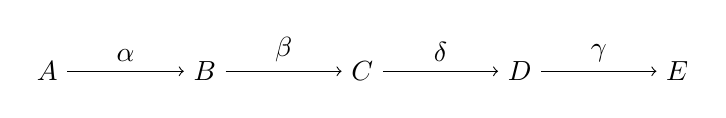
\begin{tikzpicture}[auto, node distance=2cm]
		\node(A){$A$};
		\node(B)[right of=A]{$B$};
		\node(C)[right of=B]{$C$};
		\node(D)[right of=C]{$D$};
		\node(E)[right of=D]{$E$};
		\draw[->](A) to node{$\alpha$}(B);
		\draw[->](B) to node{$\beta$}(C);
		\draw[->](C) to node{$\delta$}(D);
		\draw[->](D) to node{$\gamma$}(E);
	\end{tikzpicture}
\end{center}
where
$$\im{\alpha}=\ker{\beta},\qquad \im{\beta}=\ker{\delta},\qquad \im{\delta}=\ker{\gamma}.$$
And a \textit{short exact sequence} is an exact sequence of the form
 \begin{center}
	\begin{tikzpicture}[auto, node distance=2cm]
		\node(A){$0$};
		\node(B)[right of=A]{$A$};
		\node(C)[right of=B]{$B$};
		\node(D)[right of=C]{$C$};
		\node(E)[right of=D]{$0$};
		\draw[->](A) to node{}(B);
		\draw[->](B) to node{$\alpha$}(C);
		\draw[->](C) to node{$\beta$}(D);
		\draw[->](D) to node{}(E);
	\end{tikzpicture}
\end{center}

\begin{prop}
    Let $(E,\pi, M)$ be a smooth vector bundle.  There exists a canonical short exact sequence
     \begin{center}
	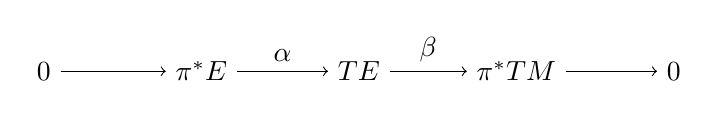
\begin{tikzpicture}[auto, node distance=2cm]
		\node(A){$0$};
		\node(B)[right of=A]{$\pi^*E$};
		\node(C)[right of=B]{$TE$};
		\node(D)[right of=C]{$\pi^*TM$};
		\node(E)[right of=D]{$0$};
		\draw[->](A) to node{}(B);
		\draw[->](B) to node{$\alpha$}(C);
		\draw[->](C) to node{$\beta$}(D);
		\draw[->](D) to node{}(E);
	\end{tikzpicture}
\end{center}
of vector bundles.
\end{prop}

\begin{proof}
Let's first unravel notation:  

Recall that
$$\pi^*E=\{(u,v)\in E\times E:\pi(u)=\pi(v)\}\cong E\oplus E,$$
and as a bundle $\pi_1:E\oplus E\to E$ with projection onto the first factor.  Post composing with $\pi$, we obtain a vector bundle $E\oplus E\to M$.

We have $(TE,\pi_E,E)$ as the usual tangent bundle of $E$, and post composing with $\pi$ we obtain a vector bundle $TE\to M$.

Let $\iota:TM\to TE$ be the zero section, and let $\pi^*TM=\iota(TM)$ denote the the subbundle of $d\pi:TE\to TM$ and then post composing with $\pi_M:TM\to M$ yields the vector bundle $\pi^*TM\to M$.

Define the map $\alpha:\pi^*E\to TE$ by
$$\alpha(u,v)=\left(p,u;0,\rest{\frac{d}{dt}}_{t=0}(u+tv)\right).$$

Define the map $\beta:TE\to \pi^*TM$ by
$$\beta(x,v;\xi,w)=(x,0;\xi,0),$$
i.e., $\beta=\iota\circ d\pi$.  Then we see that
\begin{align*}
	\beta\circ\alpha((x,v),(x,w))&=\beta\left(x,v;0,\rest{\frac{d}{dt}}_{t=0}(v+tw)\right)\\
	&=(x,0;0,0).
\end{align*}
Hence $\im{\alpha}\subseteq\ker{\beta}.$  Moreover, since $\pi^*TM$ is a rank $n$ vector bundle over $M$ and $TE$ is a rank $n+2k$ vector bundle over $M$, we have that $\ker{\beta}$ is $2k$-dimensional, as is $\im{\alpha}$ by construction.  Thus by dimensionality, we have that $\im{\alpha}=\ker{\beta}$.  Moreover, by construction $\alpha$ is injective and $\beta$ is surjective thus showing exactness.
\end{proof}


 
 
 
 
 %%%%%
 \subsection{The Vertical Bundle}
 
Let $\pi:E\to M$ and consider the associated bundle $d\pi:TE\to TM$.  Thinking of $d\pi$ as a bundle homomorphism, we have the following commutative diagram
\begin{center}
	\begin{tikzpicture}[auto, node distance=3cm]
		\node(A){$TE$};
		\node(B)[right of=A]{$TM$};
		\node(C)[below of=A]{$E$};
		\node(D)[right of=C]{$M$};
		\draw[->](A) to node{$d\pi$}(B);
		\draw[->](A) to node[swap]{$\pi_E$}(C);
		\draw[->](B) to node{$\pi_M$}(D);
		\draw[->](C) to node[swap]{$\pi$}(D);
	\end{tikzpicture}
\end{center}
In local coordinates, we have that $d\pi(x,v;\xi,w)=(x,\xi)$.  That is, for each $(x,v)\in E$, the map $d\pi_{(x,v)}:T_{(x,v)}E\to T_xM$ has constant rank $n$.  Thus $\ker{d\pi}$ is a vector subbundle of $(TE,\pi_E,E)$ where
$$(\ker{d\pi})_\theta=\ker{d\phi_\theta}.$$
Moreover, since $TE$ is a rank $n+k$ vector bundle over $E$, we have that $\ker{d\pi}$ is a rank $k$ vector subbundle by dimensionality.

We define the \textit{vertical bundle over $E$} to be
$$VE:=\ker{d\pi}.$$
The local form of a vertical vector $X\in VE$ is given by
$$X=(x,v;0,w).$$
Moreover, since the transition functions
$$d\tilde{\phi}_\alpha\circ d\tilde{\phi}_\beta^{-1}(x,v;0,w)=(\phi_{\alpha\beta}(x),\psi_{\alpha\beta}(\phi_\beta^{-1}(x))v;0,\psi_{\alpha\beta}(\phi_\beta^{-1}(x))w)$$
are linear in $(v,w)\in V\times V$ for fixed $x$, we see that $VE$ is actually a vector bundle over $M$ of rank $2k$.

Let $\iota:M\to TM$ denote the zero section of $(TM,\pi_M,M)$.  Then consider the pullback bundle $\iota^*(TE,d\pi,TM)$
\begin{center}
	\begin{tikzpicture}[auto, node distance=3cm]
		\node(A){$\iota^*TE$};
		\node(B)[right of=A]{$TE$};
		\node(C)[below of=A]{$M$};
		\node(D)[right of=C]{$TM$};
		\draw[->](A) to node{$\iota_\#$}(B);
		\draw[->](A) to node[swap]{$\iota^*d\pi$}(C);
		\draw[->](B) to node{$d\pi$}(D);
		\draw[->](C) to node[swap]{$\iota$}(D);
	\end{tikzpicture}
\end{center}
and recall that
\begin{align*}
	\iota^*TE&=\{(x,(y,v;\xi,w))\in M\times TE:\iota(x)=d\pi(y,v;\xi,w)\}\\
	&=\{(x,(y,v;\xi,w))\in M\times TE:x=y\text{ and } \xi=0\}\\
	&\cong VE.
\end{align*}
Thus we may think of the vertical bundle as the pullback via the zero section.  Moreover, we have a canonical isomorphism $\vl:E\oplus E\to VE$ given by
$$\vl(u_p,v_p)=\rest{\frac{d}{dt}}_{t=0}(u_p+tv_p).$$
In local coordinates
$$\vl((x,u),(x,v))=(x,u;0,v).$$
The map $\vl$ is called the \textit{vertical lift}.  We define the \textit{vertical projection} to be the map $\vpr:VE\to E$ given by
$$\vpr:=\pi_2\circ\vl^{-1},$$
where $\pi_2:E\oplus E\to E$, $\pi_2(u,v)=v.$  Note that
$$\pi_1\circ\vl^{-1}=\rest{\pi_E}_{VE}.$$





%%%%%
\subsection{The Double Tangent Bundle}

Consider the tangent bundle $\pi:TM\to M$ as a vector bundle in its own right.  Then from preceding remarks, we have two canonical vector bundle structures on the double tangent bundle $TTM\to TM$.  The first is as the tangent bundle to the tangent bundle given by $\pi_{TM}:TTM\to TM$.  The second is as the differential $d\pi:TTM\to TM$.

We wish to see how $(TTM, d\pi, TM)$ and $(TTM, \pi_{TM}, TM)$ are related.  To this end, define the \textit{canonical flip} $\kappa:TTM\to TTM$ given in local coordinates by
$$\kappa(x,v;\xi,\eta)=(x,\xi;v,\eta).$$
Then
$$d\pi\circ\kappa=\pi_{TM}$$
and
$$\pi_{TM}\circ\kappa=d\pi.$$
Moreover, it's clear that $\kappa^{-1}=\kappa$.

\begin{prop}
    $\kappa:TTM\to TTM$ is the unique smooth mapping such that
    $$\pfrac{}{s}\pfrac{}{t}\Gamma(s,t)=\kappa(\pfrac{}{t}\pfrac{}{s}\Gamma(s,t))$$
    for any smooth $\Gamma:\R^2\to M$.
\end{prop}

Recall that for a vector field $X\in\vf{M}$, we may treat $X$ as smooth map $X:M\to TM$, and hence we have the differential $dX:TM\to TTM$.

\begin{prop}
    For $X,Y\in\vf{M}$, we have that
    $$[X,Y]=\vpr\circ(dY\circ X-\kappa\circ dX\circ Y)$$
    and
    $$dY\circ X-\kappa\circ dX\circ Y=\vl(Y,[X,Y]).$$
\end{prop}

\begin{proof}
Recall that in local coordinates, we have that
\begin{align*}
	[X,Y]&=X[Y^j]\partial_j-Y[X^j]\partial_j\\
	&=X^i\pfrac{Y^j}{x^i}\partial_j-Y^i\pfrac{X^j}{x^i}\partial_j\\
	&=dY^j(X)\partial_j-dX^j(Y)\partial_j.
\end{align*}
Now, treating $X,Y:M\to TM$ as a smooth map, we have in local coordinates that
$$X(x)=(x,\cl{X}(x)),\qquad Y(x)=(x,\cl{Y}(x)).$$
Then as a map $dX_p:T_pM\to T_{X(p)}TM$ we have the local expression
$$dX_p=
\begin{pmatrix}
\id_{T_pM}\\
d\cl{X}_p
\end{pmatrix},$$
and hence for $Y\in TM$, we see that that
$$dX\circ Y(x)=(x,\cl{X}(x);\cl{Y}(x),d\cl{X}_x(\cl{Y}_x)).$$
It's clear from this that the first expression follows, as does the second from our local expression of vertical lift.
\end{proof}



 
 

















	



%%%%%
\section{Sprays}

Let $M$ be a smooth manifold with tangent bundle $(TM,\pi,M)$.  Let $X:TM\to TTM$ be a smooth vector field.  We say that $X$ is a \textit{differential equation of second order} or a \textit{vector field of second order} if
$$d\pi\circ\xi=\id_{TM}.$$
That is, in particular, $\xi$ is a section of $(TTM,\pi_{TM},TM)$ and of $(TTM,d\pi,TM)$.  

A differential equation of second order $X$ is called a \textit{spray of $M$} if 
$$X(sv)=ds(s(X(v)))$$
for all $s\in\R, v\in TM$, where $s:TM\to TM$, $s(x,v)=(x,sv)$, and similarly, $s:TTM\to TTM$, $s(v,\theta)=(sv,s\theta)$.

Let $(U,x)$ be local coordinates on $M$ which trivialize $TM$ and $TTM$.  Then under the usual identifications, we have that
$$TU=U\times\R^n,\qquad TTU=(U\times\R^n)\times (\R^n\times\R^n).$$
In these local coordinates, a vector field $X:TU\to TTU$ is given by
$$X(x,v)=(x,v;f(x,v),g(x,v)).$$
Now $X$ is a vector field of second order if and only if $f(x,v)=v$.

\begin{lem}
    $X(x,v)=(x,v;v,g(x,v))$ is a spray if and only if $g(x,sv)=s^2g(x,v)$ for all $s\in\R$ and $(x,v)\in U$.
\end{lem}

\begin{proof}
Noting that as a map $s:TU\to TU$, $s(x,v)=(x,sv)$, we have that $ds:TTU\to TTU$ given by
$$ds(x,v;u,w)=(x,v;u,sw).$$
Hence
\begin{align*}
	ds(s(X(x,v)))&=ds(s(x,v;v,g(x,v)))\\
	&=ds(x,sv;sv,sg(x,v))\\
	&=(x,sv;sv,s^2g(x,v))
\end{align*}
and since
$$X(x,sv)=(x,sv;sv,g(x,sv)),$$
the result then follows.
\end{proof}

Note that that the above Lemma is trivially satisfied if $g=0$.  Thus sprays exist local, and hence via a partition of unity sprays exist globally.


\begin{prop}
    Let $X\in\vf{TM}$.  Then $X$ is a vector field of second order if and only if each maximal integral curve $\beta_v:(a_v,b_v)\to TM$ with initial point $v\in TM$ and projection $\alpha_v:=\pi\circ\beta_v$ satisfies $\alpha_v'=\beta_v$.
\end{prop}

\begin{proof}
Fix $v\in TM$ and let $\beta_v$ be a maximal integral curve for $X$, and in particular, $X(v)=\beta_v'(0)=\beta_{v,*}(\rest{\frac{d}{dt}}_{t=0})$ and suppose $\alpha_v'=\beta_v$.  Then
\begin{align*}
	d\pi\circ X(v)&=d\pi\circ\beta_{v,*}\left(\rest{\frac{d}{dt}}_{t=0}\right)\\
	&=d(\pi\circ\beta_v)\left(\rest{\frac{d}{dt}}_{t=0}\right)\\
	&=d(\alpha_v)\left(\rest{\frac{d}{dt}}_{t=0}\right)\\
	&=\alpha_v'(0)\\
	&=\beta_v(0)\\
	&=v,
\end{align*}
and thus $X$ is of second order.

Conversely, suppose $X$ is of second order, and let $\beta_v$ be a maximal integral curve of $X$.  Then
\begin{align*}
	\alpha_v'(t)&=(\pi\circ\beta_v)'(t)\\
	&=d\pi\circ\beta_v'(t)\\
	&=d\pi\circ X(\beta_v(t))\\
	&=\beta_v(t),
\end{align*}
as desired.
\end{proof}

\begin{prop}
    Let $X$ be a vector field of second order.  Then $X$ is a spray if and only if its integral curves (with the previous proposition's notation) satisfies the following two properties:
    \begin{enumerate}[i.]
    \item For $s,t\in\R$ and $v\in TM$, then $st\in(a_v,b_v)$ if and only if $t\in(a_{sv},b_{sv})$.
    \item For $s,t\in\R$ and $v\in TM$ with $st\in(a_v,b_v)$, then $\alpha_v(st)=\alpha_{sv}(t)$.
    \end{enumerate}
\end{prop}

\begin{proof}
Suppose all of the integral curves of $X$ have the desired properties, and let $\beta_v$ be one such curve.  Recall that for $\alpha_v=\pi\circ\beta_v$, since $X$ is of second order, $\alpha_v'=\beta_v$.  Since $\alpha_v(st)=\alpha_{sv}(t)$ for $st\in(a_v,b_v)$, differentiating with respect to $t$, we obtain
$$s(\alpha_v'(st))=\alpha_{sv}'(t),$$
or rather
$$s(\beta_v(st))=\beta_{sv}(t).$$
Differentiating once more and using the chain rule for $s:TM\to TM$, we then obtain
$$\beta_{sv}'(t)=ds(s(\beta_v'(st))),$$
and hence at $t=0$,
$$X(sv)=\beta_{sv}'(0)=ds(s(\beta_v'(0)))=ds(s(X(v))),$$
thus showing that $X$ is a spray.

Conversely, let $\beta_v:(a_v,b_b)\to TM$ be a maximal integral curve of $X$.  Fix $s\in\R$ and define the curve $t\mapsto\gamma_v(t)$, where $\gamma_v(t)=s\beta_v(st)$ and $t$ is such that $st\in(a_v,b_v)$.  Then
\begin{align*}
	\gamma_v'(t)&=ds(s(\beta_v'(st)))\\
	&=ds(s(X(\beta_v(st))))\\
	&=X(s\beta_v(st))\\
	&=X(\gamma_v(t)).
\end{align*}
Thus $\gamma_v$ is an integral curve of $X$ with initial condition $\gamma_v(0)=sv$.  By the uniqueness of integral curves, we conclude that $\gamma_v(t)=\beta_{sv}(t)$ and that $t\in(a_{sv},b_{sv})$.  When $s\neq0$, we obtain the reverse inclusion replacing $s$ by $\frac{1}{s}$.  Moreover, if $s=0$ and $t\in(a_0,b_0)$, then we trivially have that $0\in(a_v,b_v)$ for any $v\in TM$.

Finally, for any such $s,t$ we have that
$$\beta_{sv}(t)=s\beta_v(st),$$
and taking the projection, we see that
$$\alpha_{sv}(t)=\pi\circ\beta_{sv}(T)=\pi(s(\beta_v)(st)))=\alpha_v(st).$$  
\end{proof}



\subsection{The Exponential Map}

Let $X$ be a spray on $M$.  Then define the \textit{domain of the exponential map} to be the set 
$$\mathcal{O}^X:=\{v\in TM:1\in (a_v,b_v)\}.$$
We then define the \textit{exponential map with respect to the spray $X$} to be the map $\exp:\mathcal{O}^X\to M$ given by
$$\exp(v)=\alpha_v(1),$$
where $\alpha_v:=\pi\circ\beta_v$ and $\beta_v:(a_v,b_v)\to TM$ is the maximal integral curve for $X$ with initial condition $v\in TM$.  For each $p\in M$, we also define the \textit{restricted exponential map} to be $\exp_p:\mathcal{O}_p^X\to M$ given by $\exp_p=\rest{\exp}_{\mathcal{O}_p^X}$, where $\mathcal{O}_p^X=\mathcal{O}^X\cap T_pM$.  When the spray $X$ is understand, the dependence is typically suppressed in the notation.

Recall that subset $S$ of a vector space $V$ is \textit{star-shaped with respect to $x\in V$} if for all $y\in S$, the line segment from $x$ to $y$ is contained in $S$, i.e., the curve $\psi(t):=ty+(1-t)x$ satisfies $\psi(t)\in S$ for all $t\in[0,1]$.

\begin{prop}[Properties of the Exponential Map]
    Let $M$ be a smooth manifold and let $X$ be a spray on $M$.  
    \begin{enumerate}[a.]
    	\item $\mathcal{O}$ is an open neighborhood of $TM$ containing the zero section $\iota(M)$, and each $\mathcal{O}_p$ is a star-shaped region with respect to $0$ in $T_pM$.
    	\item For each $v\in\mathcal{O}$,
    		$$\alpha_v(t)=\exp(tv)$$
    		for all $t\in(a_v,b_v)$.
    	\item $\exp:\mathcal{O}\to M$ is smooth.
    	\item For each $p\in M$, the differential $d(\exp_p)_0:T_0T_pM\to T_pM$ is the identity map on $T_pM$ under the usual identification.	
    \end{enumerate}
\end{prop}

\begin{proof}
By our rescaling properties for sprays, (b.) is immediately shown.  Moreover, since for any $v\in\mathcal{O}_p$, we have that $[0,1]\subset(a_v,b_b)$, we conclude that $[0,1]v\subset\mathcal{O}_p$ and that $\mathcal{O}_p$ is a star-shaped region with respect to $0$ in $T_pM$ for each $p\in M$.

To show that $\mathcal{O}$ is open, recall that by the Fundamental Theorem on Flows of Vector Fields, there exists an open set $\mathcal{D}\subseteq\R\times TM$ and smooth map $\theta:\mathcal{D}\to TM$ such that $(0,v)\in\mathcal{D}$ for all $v\in TM$ and $\theta(t,v)=\beta_v(t)$.

Let $v\in\mathcal{O}$, then since $(1,v)\in\mathcal{D}$ by definition, there exists an open neighborhood of $(1,v)$ in $\R\times TM$ such that $\theta$ is defined.  Therefore, there exists a neighborhood about $v\in TM$ for which $\beta_v(t)$ exists for all $t\in[0,1]$.  Thus $\mathcal{O}$ is open in $TM$.  Moreover, since $\exp=\rest{\pi\circ\theta(1,\cdot)}_{\mathcal{O}}$, we conclude that $\exp$ is smooth on $\mathcal{O}$.

Finally, let $v\in T_pM$, so we have by the corresponding isomorphism
$$k(v)=\rest{\frac{d}{dt}}_{t=0}(tv)\in T_0(T_pM).$$
Then
\begin{align*}
	d(\exp_p)_0(k(v))&=\rest{\frac{d}{dt}}_{t=0}(\exp_p(tv))\\
	&=\rest{\frac{d}{dt}}_{t=0}(\alpha_v(t))\\
	&=\alpha_v'(0)\\
	&=\beta_v(0)\\
	&=v,
\end{align*}
thus completing the proof.
\end{proof}

















	



%%%%%
\section{Constructions via Sprays}

Let $\hat{\pi}:E\to M$ be a smooth vector bundle.  Let $\iota:M\to E$ denote the zero section, and consider the pullback $\iota^*(TE,\pi_E,E)$ bundle given by $(\iota^*TE,\iota^*\pi_E,M)$.  We've seen that this is precisely the restriction $\rest{TE}_M$, and we let $\pi:\rest{TE}_M\to M$ denote this vector bundle.

It should be noted that this is not the vertical bundle since we're taking the zero section of $(E,\hat{\pi},M)$ and not $(TM,\pi_M,M)$.  If $E=TM$, then $\rest{TTM}_M$ is the canonical involution of $VTM$.

As a map $\iota:M\to E$ and so $d\iota:TM\to TE$ with $\im{d\iota}\subseteq\rest{TE}_M$.  Since $\iota$ is an embedding, $d\iota$ is a fiberwise injective bundle morphism, and hence $TM\cong\im{d\iota}$ is a subbundle of $\rest{TE}_M$.  Moreover, in local coordinates, we have that
$$d\iota(x,\xi)=(x,0;\xi,0).$$

Now define the bundle morphism $k:E\to TE$ by
$$k(v)=\vl(0,v)=\rest{\frac{d}{dt}}_{t=0}(tv),$$
and hence in local coordinates
$$k(x,v)=(x,0;0,v).$$
Thus $\im{k}\subseteq\rest{TE}_M$ and we similarly have that $k$ is an embedding.  Thus $E\cong\im{k}$ is a vector subbundle of $\rest{TE}_M$.

Finally, since $\rest{TE}_M$ consists of points in local coordinates given by $(x,0;\xi,w)$ we conclude that the map $(k,d\iota):E\oplus TM\to\rest{TE}_M$ is a vector bundle isomorphism.

With the above decomposition of the vector bundle $\pi:\rest{TE}_M\to M$, we see from construction that the vertical bundle
$$V(\rest{TE}_M)=\ker{d\pi}=\im{k}\cong E.$$
We call the other portion of this decomposition the \textit{horizontal bundle}, that is, as subbundle $H(\rest{TE}_M)\leq\rest{TE}_M$, we have that
$$H(\rest{TE}_M)=\im{d\iota}\cong TM.$$

Now, when $E=TM$, we let $VM$ and $HM$ denote the the above vertical and horizontal bundles, and have that each $VM\cong TM$ and $HM\cong TM$.  Thus by our above decomposition, we have that
$$\rest{TTM}_M=VM\oplus HM\cong TM\oplus TM.$$


Let $X$ be a spray on $M$ with exponential domain $\mathcal{O}\subseteq TM$.  Since $\mathcal{O}$ is open, we have an identical splitting of
\begin{align*}
	\rest{T\mathcal{O}}_M&=k(TM)\oplus d\iota(TM)\\
	&=TM\oplus TM.
\end{align*}
Moreover, from construction $\exp\circ\iota=\id_M$.

\begin{lem}
    The differential of the exponential map on the zero section,
    $$d(\exp)_{\iota(x)}:T_{\iota(x)}\mathcal{O}=k(T_xM)\oplus d\iota_x(T_xM)\to T_xM$$ is given by the map
    $$(v,w)\mapsto v+w.$$
\end{lem}

\begin{proof}
Fix $x\in M$, $u,v\in T_xM$, and so $d\iota_x(w)=(0,w)$ and $k(v)=(v,0)$.  Since $\exp\circ i=\id_M$, for $x\in M$, we have that
\begin{align*}
	d(\exp)_{\iota(x)}(0,w)&=d(\exp)_{\iota(x)}(d\iota_x(w))\\
	&=d(\exp\circ\iota)_x(w)\\
	&=d(\id_M)_x(w)\\
	&=\id_{T_xM}(w)\\
	&=w.
\end{align*}

On the other hand, note that $k(v)=\left(\rest{\frac{d}{dt}}_{t=0}(tv),0\right)=(v,0)$.  Then
\begin{align*}
	d(\exp)_{\iota(x)}(v,0)&=d(\exp)_{\iota(x)}\left(\rest{\frac{d}{dt}}_{t=0}(tv)\right)\\
	&=\rest{\frac{d}{dt}}_{t=0}\exp(tv)\\
	&=\rest{\frac{d}{dt}}_{t=0}\alpha_{tv}(1)\\
	&=\rest{\frac{d}{dt}}_{t=0}\alpha_v(t)\\
	&=\alpha_v'(0)\\
	&=v.
\end{align*}
That is, for $(v,w)=k(v)+d\iota_x(w)$, we have that
$$d(\exp)_{\iota(x)}(v,w)=v+w,$$
as desired.
\end{proof}

\begin{lem}
    The differential of the map $(\pi,\exp):\mathcal{O}\to M\times M$ on the zero section 
    $$d(\pi,\exp)_{\iota(x)}:T_{\iota(x)}\mathcal{O}=k(T_xM)\oplus d\iota_x(T_xM)\to T_xM\oplus T_xM$$
    is given by
    $$(v,w)\mapsto(w,v+w).$$
\end{lem}

\begin{proof}
By the previous lemma, we need only show that $d\pi_{\iota(x)}:T_{\iota(x)}\mathcal{O}=k(T_xM)\oplus d\iota_x(T_xM)\to T_xM$ is given by
$$(v,w)\mapsto w.$$
Indeed,
\begin{align*}
	d\pi_{\iota(x)}(v,w)&=d\pi_{\iota(x)}(k(v))+d\pi_{\iota(x)}(d\iota_x(w))\\
	&=d\pi_{\iota(x)}\left(\rest{\frac{d}{dt}}_{t=0}(tv)\right)+d(\pi\circ\iota)_x(w)\\
	&=\rest{\frac{d}{dt}}_{t=0}(\pi(tv))+d(\id_M)_x(w)\\
	&=\rest{\frac{d}{dt}}_{t=0}(x)+\id_{T_xM}(w)\\
	&=0+w\\
	&=w,
\end{align*}
and the result follows.
\end{proof}

Thus for all $x\in M$, by the inverse function theorem, there exists an open neighborhood $U_x\subseteq\mathcal{O}$ of $\iota(x)$ such that $\rest{(\pi,\exp)}_{U_x}:U_x\to W_x$ is a diffeomorphism, where $W_x$ is an open neighborhood of $(x,x)$ in $M\times M$.



\subsection{A Metric Space Lemma}

\begin{lem}\label{thm:metricSpaceLem}
    Let $(Z,d)$ be a metric space, and suppose $X,Y,D$ are all subspaces of $Z$ with $Y\subseteq X$ and $Y\subseteq D$.  Suppose $f:D\to X$ is a continuous function such that $\rest{f}_Y=\id_Y$.  Furthermore, assume that for each $y\in Y$, there exists $\epsilon(y)>0$ such that $\rest{f}_{B_D(y,\epsilon(y))}$ is a homeomorphism onto an open subset of $X$.  Then there exists an open subspace $U\subseteq D$ of $Y$ for which $f$ is injective.
\end{lem}

\begin{proof}
For each $y\in Y$, we have that $f(B_D(y,\epsilon(y)/2))$ is open in $X$.  Hence there exists $\epsilon'(y)>0$ such that
$$B_X(y,\epsilon'(y))\subseteq f(B_D(y,\epsilon(y)/2)),$$
and $\epsilon'(y)<\frac{\epsilon(y)}{4}.$  Thus for each $y\in Y$, define the open sets
$$U_y=\left(\rest{f}_{B_D(y,\epsilon(y)/2)}\right)^{-1}(B_X(y,\epsilon'(y)),$$
and let
$$U=\bigcup_{y\in Y}U_y.$$

Now $f$ is injective on $U$.  Indeed, assume $f(z_1)=f(z_2)=y_0$ with $z_1\in U_{y_1}, z_2\in U_{y_2}$.  In particular, we have that
$$y_0=f(z_j)\in f(U_j)\subseteq B_X(y_j,\epsilon'(y_j))\subseteq B_X(y_j,\epsilon(y_j)/4).$$
Without loss of generality, assume that $\epsilon(y_1)\geq\epsilon(y_2)$.  Hence
\begin{align*}
	d(z_2,y_1)&\leq d(z_2,y_2)+d(y_2,y_0)+d(y_0,y_1)\\
	&\leq \frac{\epsilon(y_2)}{2}+\frac{\epsilon(y_2)}{4}+\frac{\epsilon(y_1)}{4}\\
	&\leq\frac{\epsilon(y_1)}{2}+\frac{\epsilon(y_1)}{4}+\frac{\epsilon(y_1)}{4}\\
	&=\epsilon(y_1),
\end{align*}
and so both $z_1,z_2\in B_D(y_1,\epsilon(y_1))$, and since $f$ is a homeomorphism here, we conclude $z_1=z_2$.
\end{proof}

\TOX{

\begin{thm}
    Suppose $(M,g)$ is a Riemannian manifold and let $\hat{g}$ denote the Sasaki-metric on $TM$.  Let $\xi$ be any spray on $M$ with associated exponential map $\exp$.  Then there exists an open neighborhood $U$ of the zero section $M$ in $TM$ and an open neighborhood $V$ of the diagonal $\Delta(M)$ in $M\times M$ such that $(\pi,\exp):U\to V$ is a diffeomorphism.
\end{thm}

\begin{proof}
We need to modify either \cref{thm:metricSpaceLem} to $f$ being just injective on $Y$ and $f(Y)\subseteq X$ for a different metric space $(X,d')$, or compose with a new map to consider the diagonal and the zero section, the same set.
\end{proof}

}






















	



%%%%%%
\section{The Normal Bundle}

\begin{tcolorbox}
	Following \textit{Differential Manifolds} by Tammo tom Dieck.  See also the ``Flowout Theorem'' in \cite{lee2003smooth}, as I'm fairly certain the Flowout Theorem is another way to characterize the integral curves of sprays.
	
	Maybe let $I=\rest{\iota}_A=\iota\circ i$ for clarity?  Idk, fix this at some point though.
	
	\cite{borisenko1987sasaki}
\end{tcolorbox}


Let $(M,g)$ be a Riemannian manifold, and let $A\hookrightarrow M$ be a submanifold, then the differential $TA\to\rest{TM}_A$ is an injective bundle morphism, and we can regard $T_aA$ as a subspace of $T_aM$.  Let $N_aA=T_aA^\perp$ in $T_aM$.  Then we have the orthogonal product
$$T_aM=N_aA\oplus T_aA.$$
Moreover, as we obtain a subbundle $NA$ of $\rest{TM}_A$, we have the decomposition
$$\rest{TM}_A=NA\oplus TA.$$
Let $\xi$ be a spray on $M$, and let $\exp:\mathcal{O}\subseteq TM\to M$ be its exponential map.  Let $\mathcal{D}=\mathcal{O}\cap NA$, then $\mathcal{D}$ is an open neighborhood of the zero section
$$\rest{i}_A(A)\subset\mathcal{D}\subset NA.$$
Thus with respect to our decomposition of
$$T_{i(a)}\mathcal{O}=k(T_aM)\oplus di_a(T_aM),$$
into horizontal and vertical components, we then have
\begin{align*}
	T_{i(a)}(\mathcal{D})&=k(N_aM)\oplus di_a(T_aA)\\
	&\cong N_aA\oplus T_aA.
\end{align*}
Let $\exp^\perp=\rest{\exp}_{\mathcal{D}}:\mathcal{D}\to M$.  Then on the zero section $i(A)$, we have that
$$d(\exp^\perp)_{i(a)}:(v,w)=v+w,$$
but $T_aM=N_aA\oplus T_aA$, hence $d(\exp^\perp)_{i(a)}$ is the identity.

Thus for each $a\in A$, there exists a neighborhood $U_a\subseteq\mathcal{D}$ of $i(a)$ such that $\exp^\perp:U_a\to V_a$ is a diffeomorphism, where $V_a\subseteq M$ is a neighborhood of $a$.

\begin{thm}[Tubular Neighborhood Theorem]\label{thm:tublar}
    Let $(M,g)$ be a Riemannian manifold with Sasaki-metric $\hat{g}$ on $TM$.  Let $\xi$ be any spray on $M$ with associated exponential map $\exp$.  Suppose $A\subset M$ is a submanifold.  Then there exists an open neighborhood $U$ of the zero section $i(A)$ in $NA$, and an open neighborhood $V$ of $A$ in $M$ such that $\rest{\exp^\perp}_U:U\to V$ is a diffeomorphism.
\end{thm}

\begin{proof}
Let $\mathcal{D}$ denote the domain of $\exp^\perp$ in the normal bundle $NA$.  Let $d$ denote the induced distance on $TM$ from the Sasaki metric $\hat{g}$, so that $(TM,d)$ is a metric space.  Then $\mathcal{D}$ is a subspace of $TM$ containing the zero section $i(A)$.  Moreover, $i(A)$ is a subspace of $i(M)$ which is a subspace of $TM$.  Finally, we have that $i\circ\exp^\perp:\mathcal{D}\to i(M)$, where
$$i\circ\exp^\perp(i(a))=i(a),$$
so the restriction to $i(A)$ is the identity, and for each $a\in A$, there exists a open neighborhood $U_a\subseteq\mathcal{D}$ of $a$ such that $\rest{i\circ\exp^\perp}_{U_a}$ is a diffeomorphism.

Since $TM$ is a metric space, for each $a\in A$, we can find $\epsilon(a)>0$ so that $B_{\mathcal{D}}(i(a),\epsilon(a))\subseteq U_a$.  As this restriction is still a homeomorphism, we may apply \cref{thm:metricSpaceLem} directly to conclude there exists there exists an open neighborhood $U\subseteq\mathcal{D}$ of $i(A)$ for which $\rest{i\circ\exp}_U$ is a diffeomorphism onto its image in $i(M)$.  Since $i$ is diffeomorphism onto it's image, post-compositing with $i^{-1}$, the result follows.
\end{proof}

When $\xi$ is the geodesic spray, and $\exp$ our Riemannian exponential map, we say the restriction of $\exp$ to the normal bundle, the \textit{normal exponential map}.

\begin{lem}
    There exists a smooth function $\epsilon:A\to\R$ such that the $\epsilon$-neighborhood,
    $$U^\epsilon=\{(a,v)\in NA:|v|_g<\epsilon(a)\}$$
    is contained in $U$.
\end{lem}

\begin{proof}
Let $\{W_\beta:\beta\in B\}$ be a collection of locally-finite charts which cover $A$.  Then due to the trivialization of the bundle $NA\to A$, we have that 
$$i(W_\beta\cap A)=(W_\beta\cap A)\times\{0\}.$$
Since this is contained in the open set $U$, there exists $\epsilon_\beta>0$ such that
$$(W_\beta\cap A)\times D(0,\epsilon_\beta)\subseteq U,$$
where
$$D(0,\epsilon_\beta)=\{v\in N_{a_0}A: |v|_{g(a_0)}<\epsilon_\beta\},$$
for some fixed $a_0\in A$, since they're all equivalent.  Let $\{\theta_\beta:\beta\in B\}$ be a partition of unity subordinate to $\{W_\beta:\beta\in B\}$.  Define the function $\epsilon:A\to\R$ by
$$\epsilon(a)=\sum_{\beta\in B}\epsilon_\beta\theta_\beta(a).$$
Then $\epsilon$ is smooth and
$$\epsilon(a)\leq\max\{\epsilon_\beta:a\in W_\beta\},$$
showing that
$$\{a\}\times D(0,\epsilon(a))\subset U,$$
for each $a\in A$.  Then
$$U^\epsilon=\bigcup_{a\in A}\{v\in N_aA:|v|_g<\epsilon(a)\}\subseteq U,$$
as desired.
\end{proof}



\begin{cor}
    When $A\subset M$ is compact, there exists $\epsilon>0$ such that the $U$ in the above theorem can be taken to be
    $$U=\{v\in NA:|v|_g<\epsilon\}.$$
\end{cor}

\begin{proof}
Since $A$ is compact, the continuously defined $\epsilon:A\to\R$ in the above proof attains a positive minimum value, and taking the constant $\epsilon$ to be this value gives the desired result.
\end{proof}













	
	
	
	



%%%%%
\section{General Fiber Bundles}

\TOX{
This section will mostly follow \cite{kolar1999natural}, \cite{michor2008topics}, and \cite{ryan2014geometry}.
}

A \textit{fiber bundle} is a quadruple $(E,\pi, M, S)$ which consists of smooth manifolds $E$, $M$, and and $S$, and a smooth surjective submersion $\pi:E\to M$ with the requirement that for each $p\in M$, there exists an open neighborhood $U\subseteq M$ of $p$ such that $\rest{E}_U:=\pi^{-1}(U)$ is diffeomorphic to $U\times S$ via a fiber respecting diagram
\begin{center}
	\begin{tikzpicture}[auto, node distance=3cm]
		\node(A){$\rest{E}_U$};
		\node(B)[right of=A]{};
		\node(C)[right of=B]{$U\times S$};
		\node(D)[below of=B]{$U$};
		\draw[->](A) to node{$\phi$}(C);
		\draw[->](A) to node[swap]{$\pi$}(D);
		\draw[->](C) to node{$\pi_1$}(D);
	\end{tikzpicture}
\end{center}

We say $E$ is the \textit{total space}, $M$ is the \textit{base manifold}, $S$ is the \textit{model fiber}, and $\pi$ is the \textit{bundle projection}.  In practice, the fiber is usual understand from context, and so we typically denote a fiber a bundle as the mapping $\pi:E\to M$, or as s script lettering of the total space, e.g., $(E,\pi,M,S)=\mathcal{E}$.  Moreover, $(U,\phi)$ as above is called a \textit{fiber chart} or a \textit{local trivialization of $E$}.

A collection of fiber charts $\{(U_\alpha,\phi_\alpha)\}$ such that $\{U_\alpha\}$ is an open cover of $M$ is called \textit{(fiber) bundle atlas}.  If we fix such an atlas, then
$$\phi_\alpha\circ\phi_\beta^{-1}(x,p)=(x,\phi_{\alpha\beta}(p)),$$
where
$$\phi_{\alpha\beta}:U_{\alpha\beta}\times S\to S$$
is smooth and $U_{\alpha\beta}=U_\alpha\cap U_\beta$, moreover, for each $x\in U_{\alpha\beta}$, we have that $p\mapsto\phi_{\alpha\beta}(x,p)$ is a diffeomorphism of $S$. It is sometimes useful to then consider $\phi_{\alpha\beta}:U_{\alpha\beta}\to\text{Diff}(S)$, but its differentiability is a very subtle question.\footnote{See \cite{michor1988gauge} for treatment of the subtlety.}  In either form, the functions $\{\phi_{\alpha\beta}\}$ are called the \textit{transition functions} and satisfy the \textit{cocycle condition}:
$$\phi_{\alpha\beta}\circ\phi_{\beta\gamma}(x)=\phi_{\alpha\gamma}(x),\qquad x\in U_{\alpha\beta\gamma},$$
and
$$\phi_{\alpha\alpha}(x)=\id_F.$$

Given an open cover $\{U_\alpha\}$ of $M$ and a cocycle of transition functions $\{\phi_{\alpha\beta}\}$, we may construct a fiber bundle $\mathcal{E}$.

\begin{lem}
    Let $\pi:E\to M$ be a surjective submersion.  If $\pi$ is proper and $M$ is connected, then $\pi:E\to M$ is a fiber bundle.
\end{lem}

Given a fiber bundle $(E,\pi,M,S)$, we consider the differential $d\pi:TE\to TM$, and define the \textit{vertical bundle}
$$VE:=\ker{d\pi}.$$

A \textit{connection} on a fiber bundle $(E,\pi,M,S)$ is a vector-valued $1$-form $\Phi\in\Omega^1(E;VE)$ such that $\Phi\circ\Phi=\Phi$ and $\im{\Phi}=VE$.  Note that such a $\Phi\in\Omega^1(E;VE)$ is a $C^\infty$-linear map $\Phi:TE\to VE$, and since $VE\subseteq TE$ the composition makes sense.


\subsubsection{Considerations}

Recall, a topological fiber bundle is quadruple $(E,\pi,M,F)$, where $E,M,F$ are topological spaces, and $\pi:E\to M$ is a continuous surjection; along with an equivalence class of bundle atlases $\{(U_\alpha,\phi_\alpha)\}$, where $U_\alpha$ is an open cover of $M$, and $\phi_\alpha$ satisfies the trivialization criteria.

Let $G$ be a topological group, i.e., $G$ is a group with a topology so that the multiplication and inversion operations are continuous.  Let $F$ be a topological space, then we say that $G$ acts on $F$ if
$$(g_1(g_2v))=(g_1g_2)v,$$
for all $g_1,g_2\in G$ and $v\in F$.  We say that $G$ acts faithfully if for every $g\in G\setminus\{e\}$, there exists $v\in F$ such that $gv\neq v$.  We say $G$ acts freely if $gv=v$ implies $g=e$.  Note that freely acting groups (on any nonempty set) are faithful.

Let $G$ act freely on $F$.  Then $G$ is (group) isomorphic to a subgroup of $\text{Homeo}(F)$.

Given a bundle $(E,\pi,M,F)$, a $G$-atlas $\{U_\alpha,\phi_\alpha\}$ is a bundle atlas for $\mathcal{E}$ such that our transitions maps for a trivialization
$$\phi_\alpha\circ\phi_\beta^{-1}:U_{\alpha\beta}\times F\to U_{\alpha\beta}\times F,\qquad \phi_\alpha\circ\phi_\beta^{-1}(x,v)=(x\phi_{\alpha\beta}(x)v)$$
are such that $\phi_{\alpha\beta}:U_{\alpha\beta}\to G$ is continuous.  A $G$-bundle is a fiber bundle $\mathcal{E}$ with an equivalence class of $G$-atlases.  The group $G$ is called the structure group of the bundle $\mathcal{E}$.

The transition functions satisfy the following:
\begin{enumerate}[i.]
\item $\phi_{\alpha\alpha}(x)=e$,
\item $\phi_{\beta\alpha}(x)=\phi_{\alpha\beta}(x)^{-1}$,
\item $\phi_{\alpha\beta}(x)\phi_{\beta\gamma}(x)=\phi_{\alpha\gamma}(x)$,
\end{enumerate}
where property (iii.) is called the cocycle condition.  The cocycle condition allows the transition functions to determine the fiber bundle $F$.

A principle $G$-bundle is a $G$-bundle where $G$ acts on $F$ freely and transitively, and hence we may identify $G$ with $F$.











	
	


\section{Basics of Vector Bundles}

\begin{tcolorbox}
Introductory definitions follow from \cite{kolar1999natural}, \cite{lee2003smooth}, \cite{ryan2014geometry}.

Check out \cite{borisenko1991riemannian} and \cite{borisenko1987sasaki}
\end{tcolorbox}








\subsubsection{Ehresmann Connections}

\begin{tcolorbox}
See \cite{ryan2014geometry}.	
\end{tcolorbox}



Let's now generalize this notion beyond the zero section.  To this end, let $\pi:E\to M$ be a smooth vector bundles, and $\pi_E:TE\to E$, $\pi_M:TM\to M$ denote the two tangent bundles, and the usual differential $d\pi:TE\to TM$ which commutes via
\begin{center}
	\begin{tikzpicture}[auto, node distance=3cm]
		\node(A){$TE$};
		\node(B)[right of=A]{$TM$};
		\node(C)[below of=A]{$E$};
		\node(D)[right of=C]{$M$};
		\draw[->](A) to node{$d\pi$}(B);
		\draw[->](A) to node[swap]{$\pi_E$}(C);
		\draw[->](B) to node{$\pi_M$}(D);
		\draw[->](C) to node[swap]{$\pi$}(D);
	\end{tikzpicture}
\end{center}

We define the vertical bundle to be $V=\ker{d\pi}$.  That is, for each $\theta=(x,u)\in E$, we have
$$V_\theta=\ker{d\pi_\theta}.$$
Let $\pi_V:V\to E$ denote this smooth vector bundle.  Since each $V_\theta$ is isomorphic to $E_x$, we get by considering the composition of bundles $\pi\circ\pi_V$ that
$$V\cong E\oplus E.$$
Consider now the pullback bundle $\pi^*E$, that is,
\begin{align*}
	\pi^*E&=\{(\theta,\eta)\in E\times E:\pi(\theta)=\pi(\eta\}\\
	&=\{((x,u),(x,v):u,v\in E_x\}\\
	&=E\oplus E.
\end{align*}
This allows us to define the fiber-isomorphism $j:\pi^*E\to V$ via
$$j((x,u),(x,v))\mapsto\rest{\frac{d}{dt}}_{t=0}(u+tv),$$
and hence the fiber-isomorphism $k:V\to E$ via
$$k(J(x,u),(x,v))=(x,v).$$

The horizontal bundle $H$ is the subbundle of $TE$ that is complementary to $V$, that is,
$$TE=H\oplus V,$$
and hence
$$T_\theta E=H_\theta\oplus V_\theta.$$
A horizontal bundle can be completely characterized by a \textit{connection form} $\omega:TE\to TE$, as a bundle endomorphism (a $(0,2)$-tensor on $E$) and satisfies
\begin{enumerate}[i.]
	\item $\omega^2=\omega,$ and
	\item $\im(\omega)=V$.	
\end{enumerate}
Then the horizontal bundle is given by
$$H=\ker{\omega},$$
and this connection form $\omega$ can be thought as the projection onto the vertical space.

To describe such a connection form, we need the notion of a horizontal lift.  To this end, let $\gamma:I\to M$ denote a path, and we say its lift $\tilde{\gamma}:I\to E$ is a \textit{horizontal lift} if $\tilde{\gamma}'(t)\in H_{\tilde{\gamma}(t)}$ for all $t\in I$.  A path $\gamma:I\to M$, $\gamma(0)=x$, $\gamma(1)=y$ \textit{has horizontal lifts} if for every $v\in E_x$, there is a unique horizontal lift $\tilde{\gamma}:I\to E$ such that $\tilde{\gamma}(0)=v$ and $\tilde{\gamma}(1)\in E_y$.  By rescaling, this definition is equivalent to $\tilde{\gamma}(t)\in E_{\gamma(t)}$ for all $t\in I$.


If every path $\gamma:I\to M$ has a horizontal lift, we say the horizontal bundle $H$ has the \textit{horizontal lifting property} and we call $H$ an \textit{Ehresmann connection on $E$}.  We use the term connection here because horizontal lifts can be used to connect the fibers of $E$.  Indeed, let $L_\gamma(v)$ denote the image of the horizontal lift of $\gamma$ with initial points $(x,v)$.  Then we may consider $L_\gamma(v)$ as the image of a section in $\Gamma(\gamma^*E)$ (noting the difference if $\gamma$ has self-intersection points), and hence the unique horizontal lift is given by
$$\tilde{\gamma}=\gamma_\#L_\gamma(v):I\to E.$$
Hence we have the diffeomorphism (with slight abuse of notation)
$$L_\gamma:E_x\to E_y,\qquad v\mapsto (L_\gamma(v))(1).$$





\subsubsection{Tangent Bundle - Revisited}

\begin{tcolorbox}
This follows from \cite{paternain2012geodesic}, \cite{ryan2014geometry}, \cite{sakai1996riemannian}.
\end{tcolorbox}


Suppose now that $(M,g)$ is a Riemannian manifold, and we have the tangent bundle $\pi:TM\to M$, and our double tangent bundle $d\pi:TTM\to TM$.  Our vertical space $V$ is defined as usual
$$V_\theta=\ker{d\pi_\theta},\qquad \theta\in TM.$$
Since $(M,g)$ is Riemannian, let $\nabla$ denote the Levi-Civita connection, and for a smooth curve, let $P^\gamma_t:T_{\gamma(0)}M\to T_{\gamma(t)}M$ denote the linear isomorphism of parallel translation along $\gamma$.  For $\theta=(x,v)\in TM$, define the \textit{horizontal lift} $L_\theta:T_xM\to T_\theta TM$ as follows:  Let $X\in T_xM$, let $\gamma:I_\epsilon\to M$ be any curve with $\gamma(0)=x$, $\gamma'(0)=X$, and consider the parallel translation $P_t^\gamma(v)$.  Then we have a curve $\alpha:I_\epsilon\to TM$ given by
$$\alpha(t)=(\gamma(t),P_t^\gamma(v)).$$
With a slight abuse of notation, we can consider $t\mapsto P_t^\gamma(v)$ a section of $I\to\gamma^*TM$, and thus define
$$L_\theta(\gamma'(0))=\rest{\frac{d}{dt}}_{t=0}P_t^\gamma(v).$$
Note that $L_\theta$ is well-defined (i.e., independent of choice of $\gamma$).  Indeed, in coordinates, let
$$X=X^i\pfrac{}{x^i},\qquad \alpha(t)=\xi^i(t)\rest{\pfrac{}{x^i}}_{\gamma(t)}.$$
Since $\alpha$ is parallel along $\gamma$, we have that
$$\nabla_{\gamma'(t)}\alpha(t)=0.$$
In particular,
\begin{align*}
0&=\rest{(\nabla_{\gamma'(t)}\alpha(t))^k}_{t=0}\\
&=\rest{\left(\nabla_{\gamma'(t)}\left(\xi^j(t)\rest{\pfrac{}{x^j}}_{\gamma(t)}\right)\right)^k}_{t=0}\\
&=\rest{\nabla_{\gamma'(t)}\xi^k}_{t=0}+\rest{\left(\xi^j(0)\nabla_{\gamma'(t)}\rest{\pfrac{}{x^j}}_{\gamma(t)}\right)^k}_{t=0}\\
&=\dot{\xi}^k(0)+\xi^j(0)\dot{\gamma}^i(0)\Gamma_{ij}^k\\
&=\dot{\xi}^k(0)+\xi^j(0)X^i\Gamma_{ij}^k,
\end{align*}
and so
$$\dot{\xi}^k(0)=-\xi^j(0)X^i\Gamma_{ij}^k.$$
Letting $v^i=\xi^i(0)$, we get that
\begin{align*}
\alpha'(0)&=(x^k, v^k, X^k, \cdot{\xi}^k(0))\\
&=(x^k, v^k, X^k, -v^iX^j\Gamma_{ij}^k).
\end{align*}
That is,
$$L_{(x,v)}(X)=(x^k,v^k,X^k,-v^iX^j\Gamma_{ij}^k),$$
independent of choice of curve.

Now for $\theta\in TM$, we can define the horizontal subspace
$$H(\theta)=L_\theta(T_xM).$$

Since
$$d\pi(x^i,v^i,X^i,\eta^i)=(x^i, X^i),$$
we clearly have that
$$d\pi_\theta\circ L_\theta=\id_{TpM},$$
and hence $V(\theta)\cap H(\theta)=\{0\}$.  Since both are $n$-dimensional, we have the decomposition
$$T_\theta TM=H(\theta)\oplus V(\theta).$$

Thus in coordinates, if $(x^i,v^i,X^i,\eta^i)\in T_\theta TM$, we get the decomposition
$$(x^i,v^i,X^i,\eta^i)=(x^i, v^i, X^i, -v^jX^k\Gamma_{jk}^i)+(x^i, v^i,0, \eta^i+v^jX^k\Gamma_{jk}^i).$$

Now, define the connection map $K:TTM\to TM$ as follows:  For $\theta=(x,v)\in TM$ and $\eta=(X,\eta)\in T_\theta TM$, identify $I_\theta:T_\theta T_xM \congto T_xM,$ $ I_\theta(x^i,v^i,0,\eta^i)=(x^i,\eta^i)$ and define
$$K_\theta(\eta)=I_\theta(\eta_v)=(x^i,\eta^i+v^jX^k\Gamma_{jk}^i),$$
where $\eta=\eta_h+\eta_v$ in the dirct sum.  

Note that
\begin{align*}
K_\theta\circ L_\theta(X)&=K_\theta(x^i, v^i, X^i, -v^jX^k\Gamma_{jk}^i)\\
&=I_\theta(x^i,v^i,0,0)\\
&=0.
\end{align*}

An equivalent definition to $K:TTM\to TM$ is as follows:  Fix $\theta\in TM$ and $\xi\in T_\theta TM$.  Let $\alpha:I_\epsilon\to TM$ be a curve with $\alpha(0)=\theta$ and $\alpha'(0)=\xi$.  Then $\alpha(t)=(\gamma(t),Z(t))$.  Then define
$$K_\theta(\xi)=\rest{(\nabla_{\gamma'(t)}Z(t))}_{t=0}.$$

We know define the \textit{Sasaki metric} $\hat{g}$ on $TM$.  For $\theta\in TM$ and $\xi,\eta\in T_\theta TM$, define
$$\hat{g}_\theta(\xi,\eta)=g_{\pi(\theta)}(d\pi_\theta(\xi),d\pi_\theta(\eta))+g_{\pi(\theta)}(K_\theta(\xi),K_\theta(\eta)).$$
























\section{Principle Bundles}

\TOX{
See \cite{bishop2011geometry} Chapter 3 and 5. And \cite{kobayashi1996foundations}.
}










	
	
	
	\bibliographystyle{plain}
	\bibliography{../../texInput/Bibliography}

	
\end{document}
